\documentclass{deime}
\usepackage[dvipdfmx]{graphicx}
%\usepackage{latexsym}
%\usepackage{txfonts}
%\usepackage[fleqn]{amsmath}
%\usepackage[psamsfonts]{amssymb}
%\usepackage[deluxe]{otf}
\usepackage{caption}

% 印刷位置調整 %
% 必要に応じて値を変更してください.
\hoffset -10mm % <-- 左に 10mm 移動
\voffset -10mm % <-- 上に 10mm 移動

\usepackage{enumitem,amssymb}
\newlist{todolist}{itemize}{2}
\setlist[todolist]{label=$\square$}
\usepackage{pifont}
\newcommand{\cmark}{\ding{51}}%
\newcommand{\xmark}{\ding{55}}%
\newcommand{\done}{\rlap{$\square$}{\raisebox{2pt}{\large\hspace{1pt}\cmark}}%
\hspace{-2.5pt}}

\papernumber{DEIM Forum 2019 A5-2}

\etitle{Find Target Data Fast! A Method and Its Behavior of Target
Data Collection using Online Machine Learning}
%\esubtitle{Subtitle} <- uncomment if you need subtitle.
\authorlist{%
 \authorentry[li.ruide@dl.soc.i.kyoto-u.ac.jp]{李 瑞徳}{Ruide Li}{KU}%
 \authorentry[yamakata@hal.t.u-tokyo.ac.jp]{山肩 洋子}{Yoko Yamakata}{TU}%
 \authorentry[tajima@i.kyoto-u.ac.jp]{田島 敬史}{Keishi Tajima}{KU}%
}
\affiliate[KU]{}
 {Kyoto University\\
  36-1 Yoshida-Honmachi, Sakyo-ku, Kyoto 606-8501 Japan}
\affiliate[TU]{}
 {The University of Tokyo\\
  7-3-1 Hongo, Bunkyo-ku, Tokyo 113-8656 Japan}

%\MailAddress{$\dagger$hanako@deim.ac.jp,
% $\dagger\dagger$\{taro,jiro\}@jforum.co.jp}

\begin{document}
\pagestyle{empty}

\begin{eabstract}
In this paper, we discuss a problem of collecting data of a target
class from a fixed pool of unlabeled dataset as fast as possible.  Our
method consists of two phases.  In the first phase, we repeatedly
choose a candidate data and query human annotators for the label.
During that, we use the obtained labeled data also for training a
classifier, and use it to choose the next candidate.  When the
classifier has been trained enough, we switch to the second phase.  We
apply the obtained classifier to the remaining data to collect target
data.
%
In the first phase, we want to choose candidates which are most likely
to be target data in order to collect them fast.  For the second
phase, however, we want to query a label for a data which is likely to
improve the classifier.  We have a dilemma between these two.  Another
issue is difficulty of the estimation of the accuracy of the obtained
classifier.  The labeled data set obtained in the first phase is
biased towards the target class, and by using that we need to estimate
the accuracy of the current classifier for the remaining data which is
biased in the opposite way.
%
In this paper, we explain the difficulty of this new problem by using
our experimental results, and also show the behavior of our simple
method of ballancing the dilemma explained above.
\end{eabstract}

\begin{ekeyword}
active learning, annotation, crowdsourcing, learn-to-enumerate
\end{ekeyword}

\maketitle

\section{Introduction}
\label{sec:intro}

In the pool-based active learning problem \cite{survey}, we usually
have a pool of unlabeled data, and the learner pick up a sample from
the pool for human annotation, referring to a function which gives the
priority of every sample.  In this paper, we discuss a slightly
different problem: a problem of collecting data of a target class from
a fixed pool of unlabeled dataset as fast as possible by using machine
learning but without any prelabeled training data.  We propose a
method which consists of two phases.  In the first phase, we choose a
candidate data one by one, and repeatedly query human annotators for
the label.  If it is labeled as the target class, we store it as a
target data.  During the first phase, we use the obtained labeled data
also for train a classifier, and use the classifier to choose the next
candidate.  When we determine that the classifier has been trained
enough, we switch to the second phase: we switch from human annotation
to prediction by the classifier.  We apply the obtained classifier to
the remaining unlabelled data and collect data predicted as the target
class.

This problem is different from the ordinary active learning problem in
several ways.  First, our goal is to collect target data as fast as
possible (i.e., with as few queries for non-target data).  In the
first phase, therefore, we want to choose a candidate which is most
likely to be of the target class from the remaining unlabelled data.
The performance of the obtained classifier is not important as long as
we can collect target data fast.  Moreover, the classification
boundary of the classifier is not important in our problem as long as
the single best candidate chosen by the classifier in each step is
always a target data.  On the other hand, in the ordinary active
learning, we want to achieve high accuracy of the classifier while
minimizing the total number of both target and non-target queries.  In
the ordinary active learning, therefore, uncertainty sampling
\cite{uncertainty}, in which samples with lower confidence will be
annotated earlier, is a well-known approach.  Existing research has
shown that the opposite approach, which gives higher priority to
samples with higher confidence, is a better strategy \cite{enumerate}
if we simply want to collect target data as fast as possible.

For the second phase, however, we also want to achieve high accuracy
of the classifier.  As a result, we have a dilemma between querying a
label for a data which is likely to be a target data and querying for
a data which is likely to improve the classifier.  Another issue in
this problem is difficulty of the estimation of the accuracy of the
obtained classifier on the remaining data.  Because we choose data
likely to be a target data in the first phase, our labeled data set
obtained in the first phase is biased towards the target class.  On
the contrary, the remaining data is biased towards the non-target
classes.  In order to know on what point we can trust the classifier
and switch from human annotation to the obtained classifier, we need
to estimate the accuracy of the current classifier on the remaining
biased data only by using the currently available labeled data, which
is biased in the opposite way.

We call this problem target-extraction-learning problem.  An example
scenario of a potential application is as follows.  Suppose we have a
natural disaster, and we want to collect tweets on Twitter asking for
rescue as fast as possible.  Because we cannot examine all the tweets,
we want to train a classifier, but the characteristics of tweets
asking rescue is different from disaster to disaster, and we do not
have any labeled data sets or pretrained classifiers.  We need to
label the data first, but it is waste of time to randomly sample
tweets from Twitter and ask the annotators to label them.  We should
first examine tweets that are the most likely to be relevant, and if
it is asking for rescue, we should send the rescue as soon as
possible.  We repeat it, and after obtaining enough labeled data, we
should switch to the prediction by the classifier because human
judgement takes longer time than the classifier for a huge number of
tweets.  Another example scinario is to find high risk patients among
a big group of people without existing labeled data to train a
predictive model, and under the constraint of a limited number of
checkups we can perform \cite{predictive}.

In this paper, we introduce this new problem, and explain the
difficulty of the problem by using our experimental results.  We
simulate the scinario with SVM implementation on document
classification tasks and analyze the behavior of the classifier
obtained at each step.  We also discuss how to control the
dilemma mentioned before, suggest a simple method of ballancing the
dilemma explained above, and show its behavior in our simulation.

The rmainder of the paper is organized as follows.  In the following
section, we first discuss several related literatures about active
learning and also about learning-to-enumerate problem, which is a
problem similar to our target-extraction-learning problem.  We then
define the details of our problem in Section~\ref{sec:problem}, and
propose an approach trying to provide possible solution to the problem
in Section~\ref{sec:method}.  In the experiment section, we simulate
our framework on both balanced and unbalanced data, and report the
results.  Finally, we discuss what we can conclude from the
experiments and further issues to the mentioned problems.

\section{Related Work}
\label{sec:related}

Two most important problems related to our problem is active learning
and learning-to-enumerate.  In this section, we breifly explain
existing research on these two problems.

\subsection{Active Learning \cite{survey2}}

As the boosting development of supervised machine learning, models are
becoming more and more hungry for labeled training data. As we all
know, human annotation may cost a huge amount of money and time. To
handle this problem, many active learning algorithms have been
developed. In the survey paper by Settles \cite{survey2}, the author
summarized three typical categories of active learning algorithm:
pool-based (the learner picks up a sample from the pool of unlabeled
data by means of a querying function), stream-based (the learner tells
whether to do annotation in a stream of unlabeled data) and membership
queries (the learner generates data from the feature space of
unlabeled data).

The problem in this research is close to the pool-based active
learning, especially in the aspect of a fixed pool of unlabeled data
which do not change during the annotation phase. On the other hand,
typical active learning only focus on the performance of the model,
while in our research, we try to ballance the performance of the model
which is used in the second phase, and quick collection of target data
in the first phse.

Another difference between the ordinary problem setting in active
learning and our problem setting is the assumption on the properties
of the remaining data.  In the ordinary active learning, while we
assume a closed data set when we select samples to label, we assume an
open data set when we measure the performance of the obtained model.
We assume that the selection of samples to label do not affect the
properties of the remaining data.  On the other hand, in our problem,
we assume that the selection of samples in preference to the target
data results in the remaining data biased towards the non-target data.

\subsection{Learning to Enumerate \cite{enumerate}}

Sometimes we want to find data satisfying some particular conditions
and our goal is to find such data from the whole dataset as fast as
possible.  One scenario might be to find
% high risk patients from a big group of people.
tweets asking for rescue after some natural disaster, ex explained
before.

In such a case, if we have an extensive labeled dataset to train our
model in advance, the best strategy would be to train a model with it
and to solely rely on the predictions by the model to identify all
data of the target class.  However, when we do not have any labeled
data in adnvance, one approach is to construct a training set while
examining data that are most likely to be the target data one by one,
and use the current trained model to choose the next candidate.  In
other words, we can continue the first phase of our method until we
find all the target data.  In this setting, we have a dilemma between
querying a label for a data which is likely to be a target data and
querying for a data which is likely to improve the classifier, as
explained before.  J\"{o}rger et al.\ \cite{enumerate} call this
problem the learning-to-enumerate problem.

This is a typical exploitation vs. exploration dilemma that has been
studied extensively in reinforcement learning. J\"{o}rger et al.\
\cite{enumerate} proposed a simple $\epsilon$-greedy like strategy,
and tested it with different base learners and heuristic functions, on
19 small and medium-sized public datasets accessible through the UCI
Machine Learning Repository.  The results of their experiments shows
that the best result was achieved by an exploitation only ($\epsilon$
= 0) strategy.  Here the exploitation means the model picks up a data
that is the most likely to be of the target class, i.e., the data for
which the model has the highest confidence.

However, there is a difference in our research from their
learning-to-enumerate problem.  Their purpose is to find all target
data by human labeling, while in our research, we want to switch to
the prediction by the model at certain point, when we can be sure that
the model is well trained.

\section{Problem Definition}
\label{sec:problem}

In target-extraction-learning problem, as the literal meaning, we want
to extract target data faster, and also try to learn a model. We
presume that there is a fixed pool of unlabeled data, and the final
purpose is to find target samples using as few non-target annotation
as possible. To achieve this goal, we consider two-phase method. At
the early phase, the system choose data that are likely to be target
data, query for human annotation, and train a model with labeled
data. At the later phase, we switch from human annotation to the
prediction by the model, and provide a ranking of data based on the
likelihood of being a target data.

At the early phase, it is reasonable just to make use of the
learning-to-enumerate algorithm, but the point is that, the labeled
data, which is used to train a machine learning model, is biased
towards target samples, so we can not estimate how the model will
perform on the unlabeled data. In order to know the details, we build
a framework to simulate this annotation process.

\begin{figure}[!t]
\centering
\includegraphics[width=0.5\textwidth]{resource/structure}
\captionof{figure}{Flow Chart of Simulation Process}
\label{structure}
\end{figure}

A flow chart of the simulation process is shown in
Figure~\ref{structure}. The framework works as follows:
\begin{itemize}
\item Iteratively pick up a sample from the unlabeled data pool at
each step according to a certain policy (similar to querying function
in active learning).
\item We usually use all labeled data to train the model, but in this
framework, we split a small part of labeled pool as ``current test
set'', to evaluate the model at each step.  Metrics, such as precision
and recall, measured on this current test set are available in real
application.
\item In comparison, we provide a test set with label to evaluate the
model without bias, which we call it ``oracle test set''.  Various
metrics mesured on the oracle test set are only available in this
simulation for research purpose, and cannot be known in real
application.
\item Use the labeled data pool to train a machine learning model, and
use the model to update the querying function if needed.
\end{itemize}

\subsection{Evaluation}
In order to see every detail in the annotation simulation, we evaluate
several metrics. Note that there are metrics that we can obtain in
real application, and metrics that we cannot obtain in real
application.  In the list below, for the metrics that can be known in
real application, the corresponding checkbox is checked.  The others
are used only for the evaluation in this simulation.

\begin{todolist}
  \item Accuracy, recall, precision and f1-score on oracle test set.
  \item[\done] Accuracy, recall, precision and f1-score on current test set.
  \item Positive coverage: the ratio of retrieved target samples to all target samples.
  \item[\done] Recent labeled target proportion: the proportion of
  retrieved target samples in recent K labeled samples.
  \item R-precision on unlabeled data.
\end{todolist}

We need an explanation on the last one in the list above, i.e.,
R-precision.  We want the model to be able to give a target likelihood
ranking of the remaining unlabeled data.  To measure that ability of
the model, we use R-precision.  R-precision on the remaining data is
defined as follows:
%
\[
\mbox{\rm R-precision} = \frac{A}{R}
\]
%
where $R$ is the number of target data in the remaining data, and $A$
is the number of target data ranked within top-$R$ by the model.
However, if we use the ordinary R-precision to measure the performance
of the model on the remaining data, the comparison can be unfair.  For
example, if we have been very successful in collecting target data and
only a small number of difficult-to-find samples are left in the
remaining data, it is difficult to achieve high R-precision on that
remaining data.  On the contrary, if we have been unsuccessful and
many target data is still left in the remaining data, it is easier to
achieve high R-precision on the remaining data.  To avoid this
unfairness, we add the number of already-found target samples to both
numerator and dominator of R-precision.  That is, we use R-precision
defined by the formula below:
\[
\mbox{\rm R-precision} = \frac{A+F}{R+F}
\]
where $F$ is the number of already-found target data.

Metrics on oracle test set are used to give the ``real'' performance
of obtained model in this simulation, and metrics on current test set
are used to estimate the performance of the model on the remaining
data in real applications (since oracle test set is not available
there). At the early phase, we evaluate the performance of finding
target data by positive coverage. At the later phase, we use
R-precision defined above to evaluate the target likelihood ranking of
unlabeled data predicted by the obtained model.

\section{Proposed Approaches}
\label{sec:method}

In target-extraction-learning, we have a dilemma that it is hard to
let these two purposes (improving the model and finding target data
fast) be fulfilled at the same time.  The reason is that if we find
target data faster, the data used to train the model becomes biased
towards target data, and as a result, the performance of the model
will be deteriorated compared with the training with random sampling.

To handle this dilemma, we propose a compromised approach that uses a
``warm'' start with random sampling to balance the trade-off.  We use
random sampling only at the very beginning of the first phase (for
example, 1/10 of the whole unlabeled pool), and switch to
target-extraction after that. The point is that, we can make use of
random sampling phase to estimate the distribution of target data in
the unlabeled pool.

Another issue in our problem is the difficulty of estimating the
accuracy of the obtained model on the remaining data due to the bias
in the training data set and the remaining data set.  To estimate the
performance of obtained model, we observe the curves of metrics on
oracle test set and current test set, and have found a regular
phenomena of ``current precision pit'', which is able to indicate the
relation between oracle and current test set.  We will explain the
details in the next section reporting our experimental results.

\section{Experiments}
\label{sec:experimtnt}

In experiments, we run simulations both on balanced data and
unbalanced data, and compared our methods with random sampling.  The
data sets we used in our experiments are as follows:

\begin{itemize}
\item Dataset 1: Text message spam classification, 1500 messages, 50\% target data (spam).
\item Dataset 2: Moive review sentiment classification, 4000 reviews, 20\% target data (positive reviews).
\end{itemize}

For machine learning model, we chose Support Vector Machine (SVM). We
have also compared Long Short Term Memory (LSTM) and Random Forest
(RF). The results showed that the linear SVM and LSTM give the similar
performance, while SVM is far more efficient to train. RF gives poor
performance without hyper-parameter tuning, but we cannot tune
hyper-parameters in real application, so we finally chose linear SVM
with all default hyper-parameters in scikit-learn library
\cite{sklearn}. In addition, we use class weight in training, as the
data could be unbalanced.

On oracle test set, we use 5-fold cross-validation in order to obtain
stable results.  On current test set, we do not use cross-validation
due to efficiency reason.

Figure~\ref{oracle1} to \ref{recent2} show the metrics observed in our
simulations.  The horizontal axis represents the size of the labeled
pool, also can be considered as ``steps''.  We use the
learning-to-enumerate algorithm \cite{enumerate} as pure
target-extraction baseline, and also use the method that combine it
with 10\% random sampling warm start.  At each step, random sampling
picks up a sample randomly, while target-extraction picks up a sample
which has the largest distance to the decision boundary on the target
side, in contrast to uncertainty sampling, which picks up a sample
closest to the boundary.

\begin{figure*}[!t]
\centering
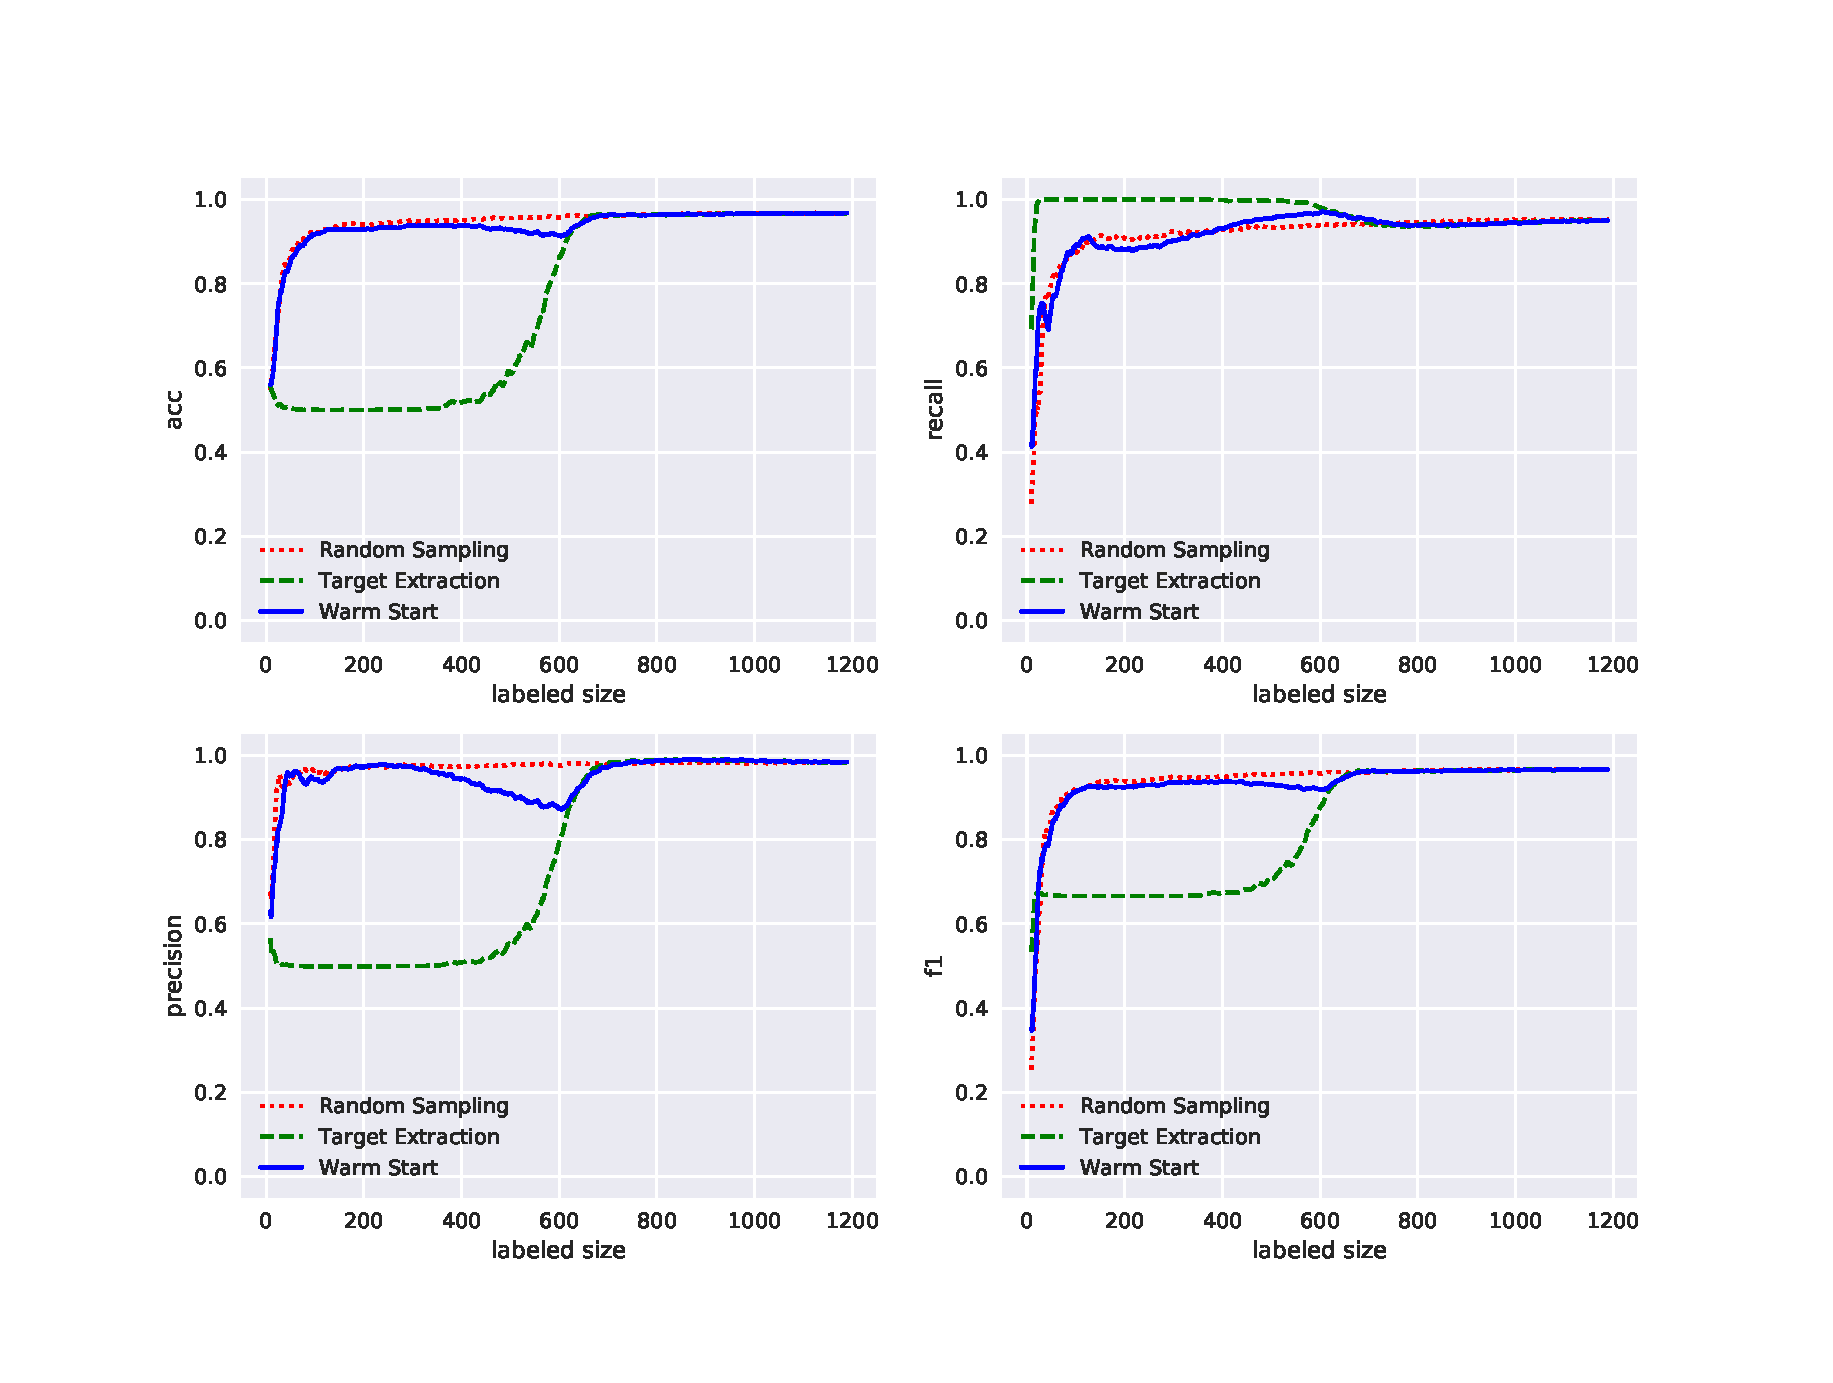
\includegraphics[width=0.9\textwidth]{resource/text_msg/oracle_k-fold5}
\captionof{figure}{Metrics on Oracle Test Set}
\label{oracle1}
\end{figure*}

\begin{figure*}[!t]
\centering
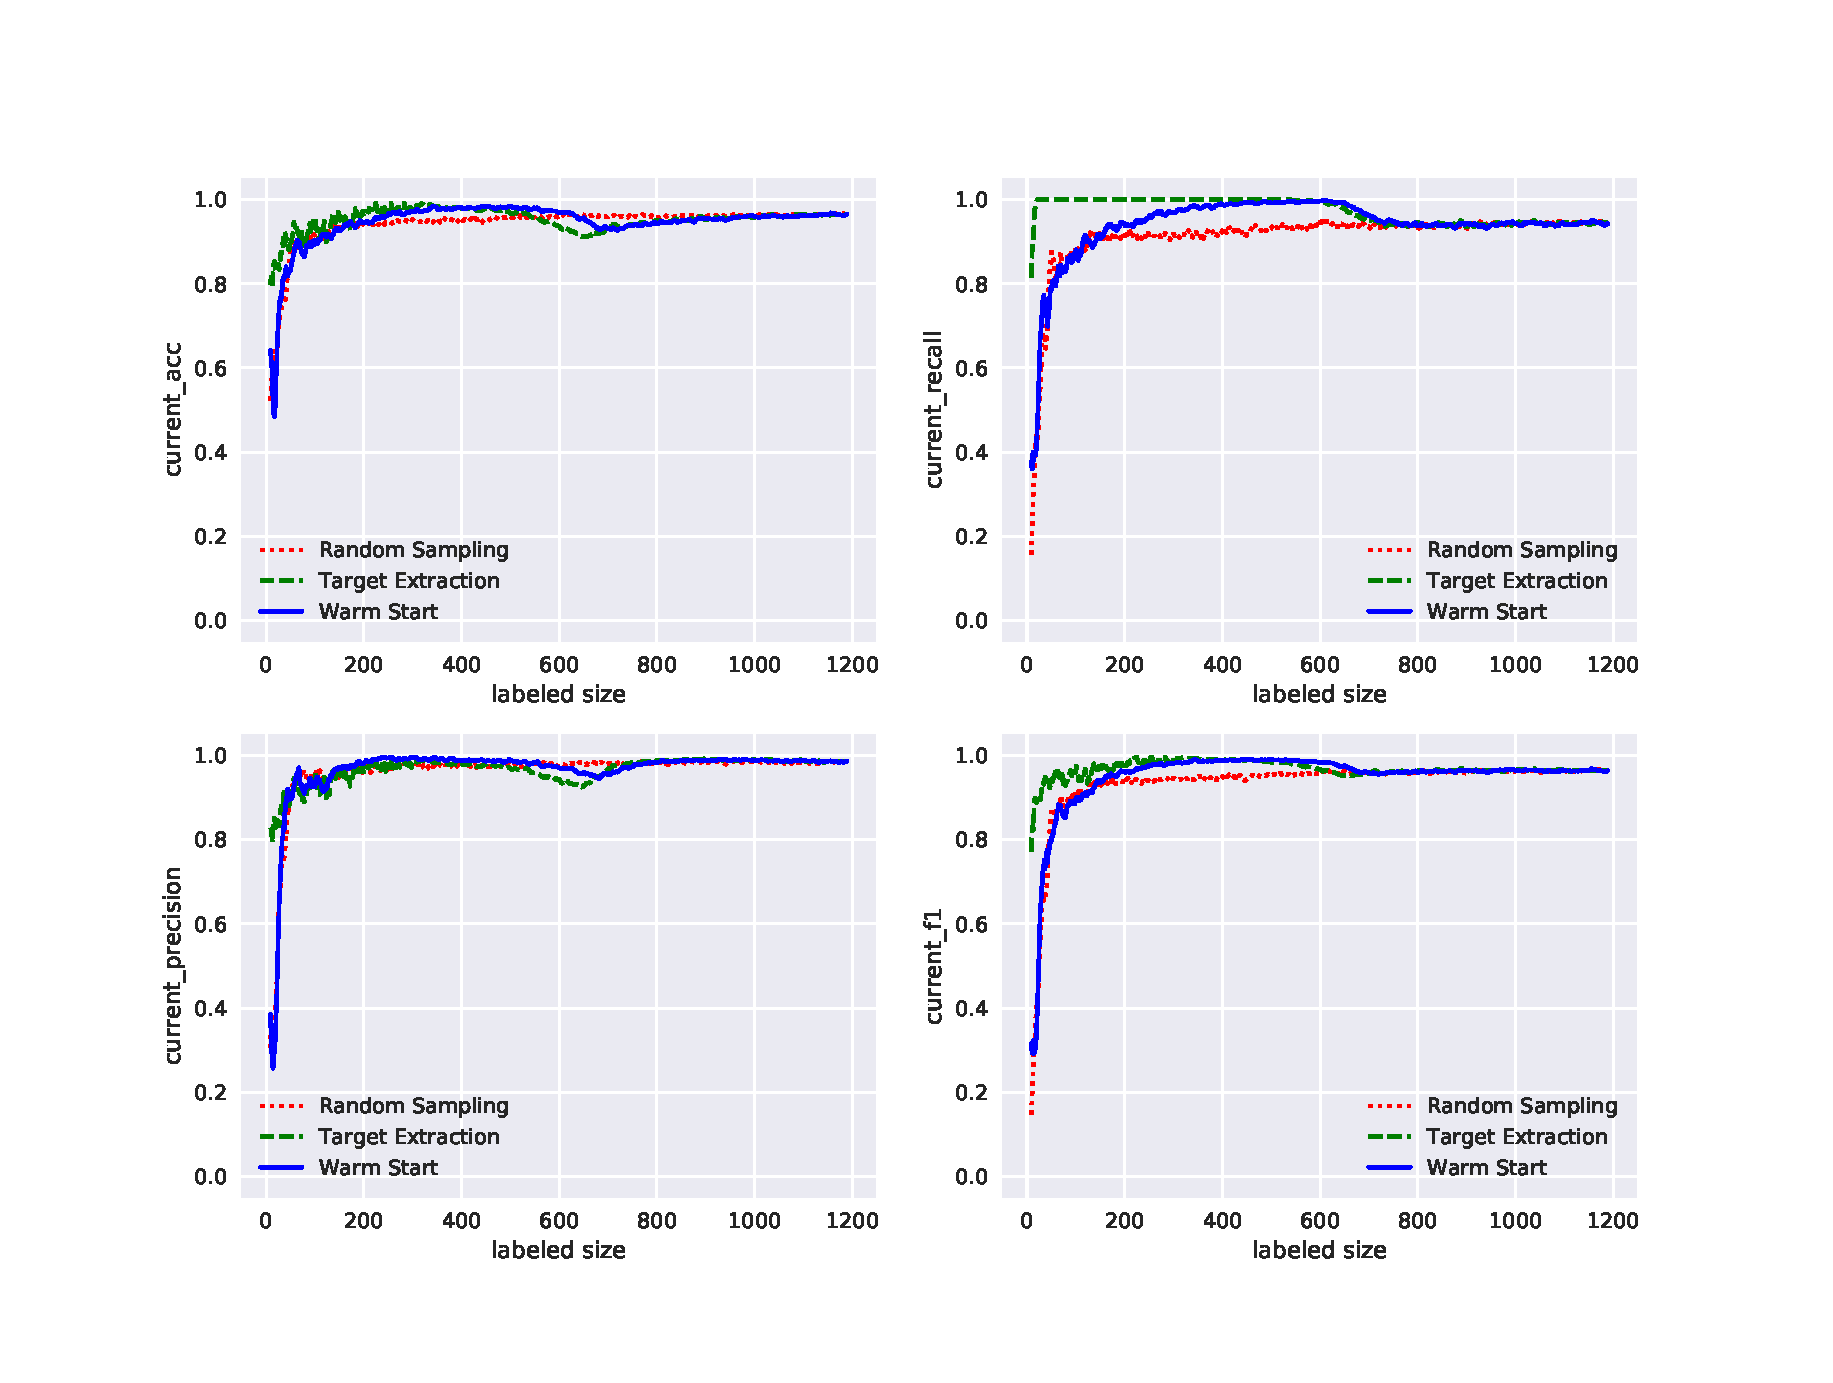
\includegraphics[width=0.9\textwidth]{resource/text_msg/current_k-fold5}
\captionof{figure}{Metrics on Current Test Set}
\label{current1}
\end{figure*}

\begin{figure}[!t]
\centering
\includegraphics[width=0.4\textwidth]{resource/text_msg/pos_coverage}
\captionof{figure}{Positive Coverage}
\label{pos_cov1}
\end{figure}

\begin{figure}[!t]
\centering
\includegraphics[width=0.4\textwidth]{resource/text_msg/r_precision}
\captionof{figure}{R-Precision}
\label{rprecision1}
\end{figure}

\begin{figure}[!t]
\centering
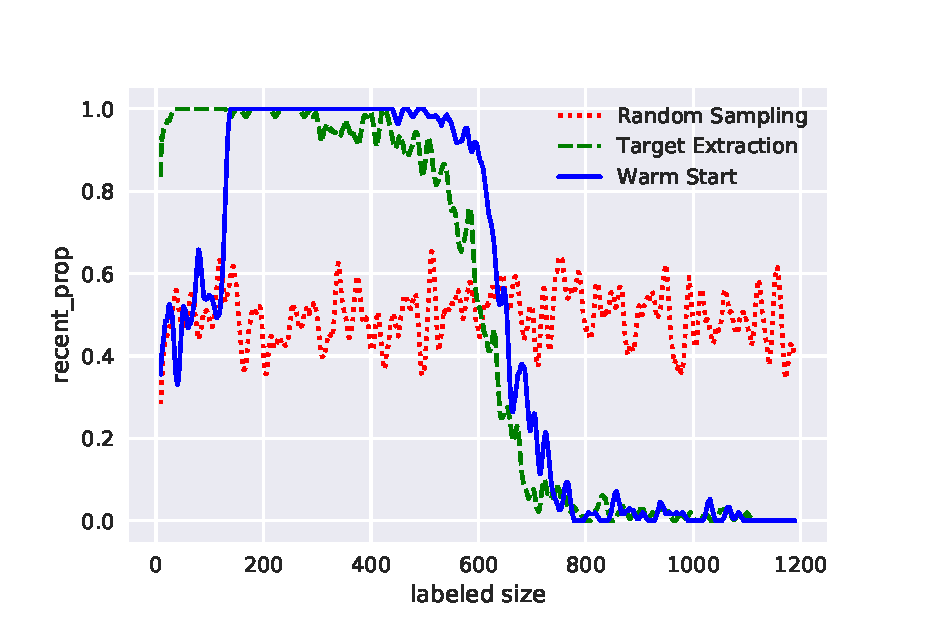
\includegraphics[width=0.4\textwidth]{resource/text_msg/recent_prop}
\captionof{figure}{Recent Target Proporttion}
\label{recent1}
\end{figure}

%%%%%%%%%%%%%%%%%%%%%%%%%

\begin{figure*}[!t]
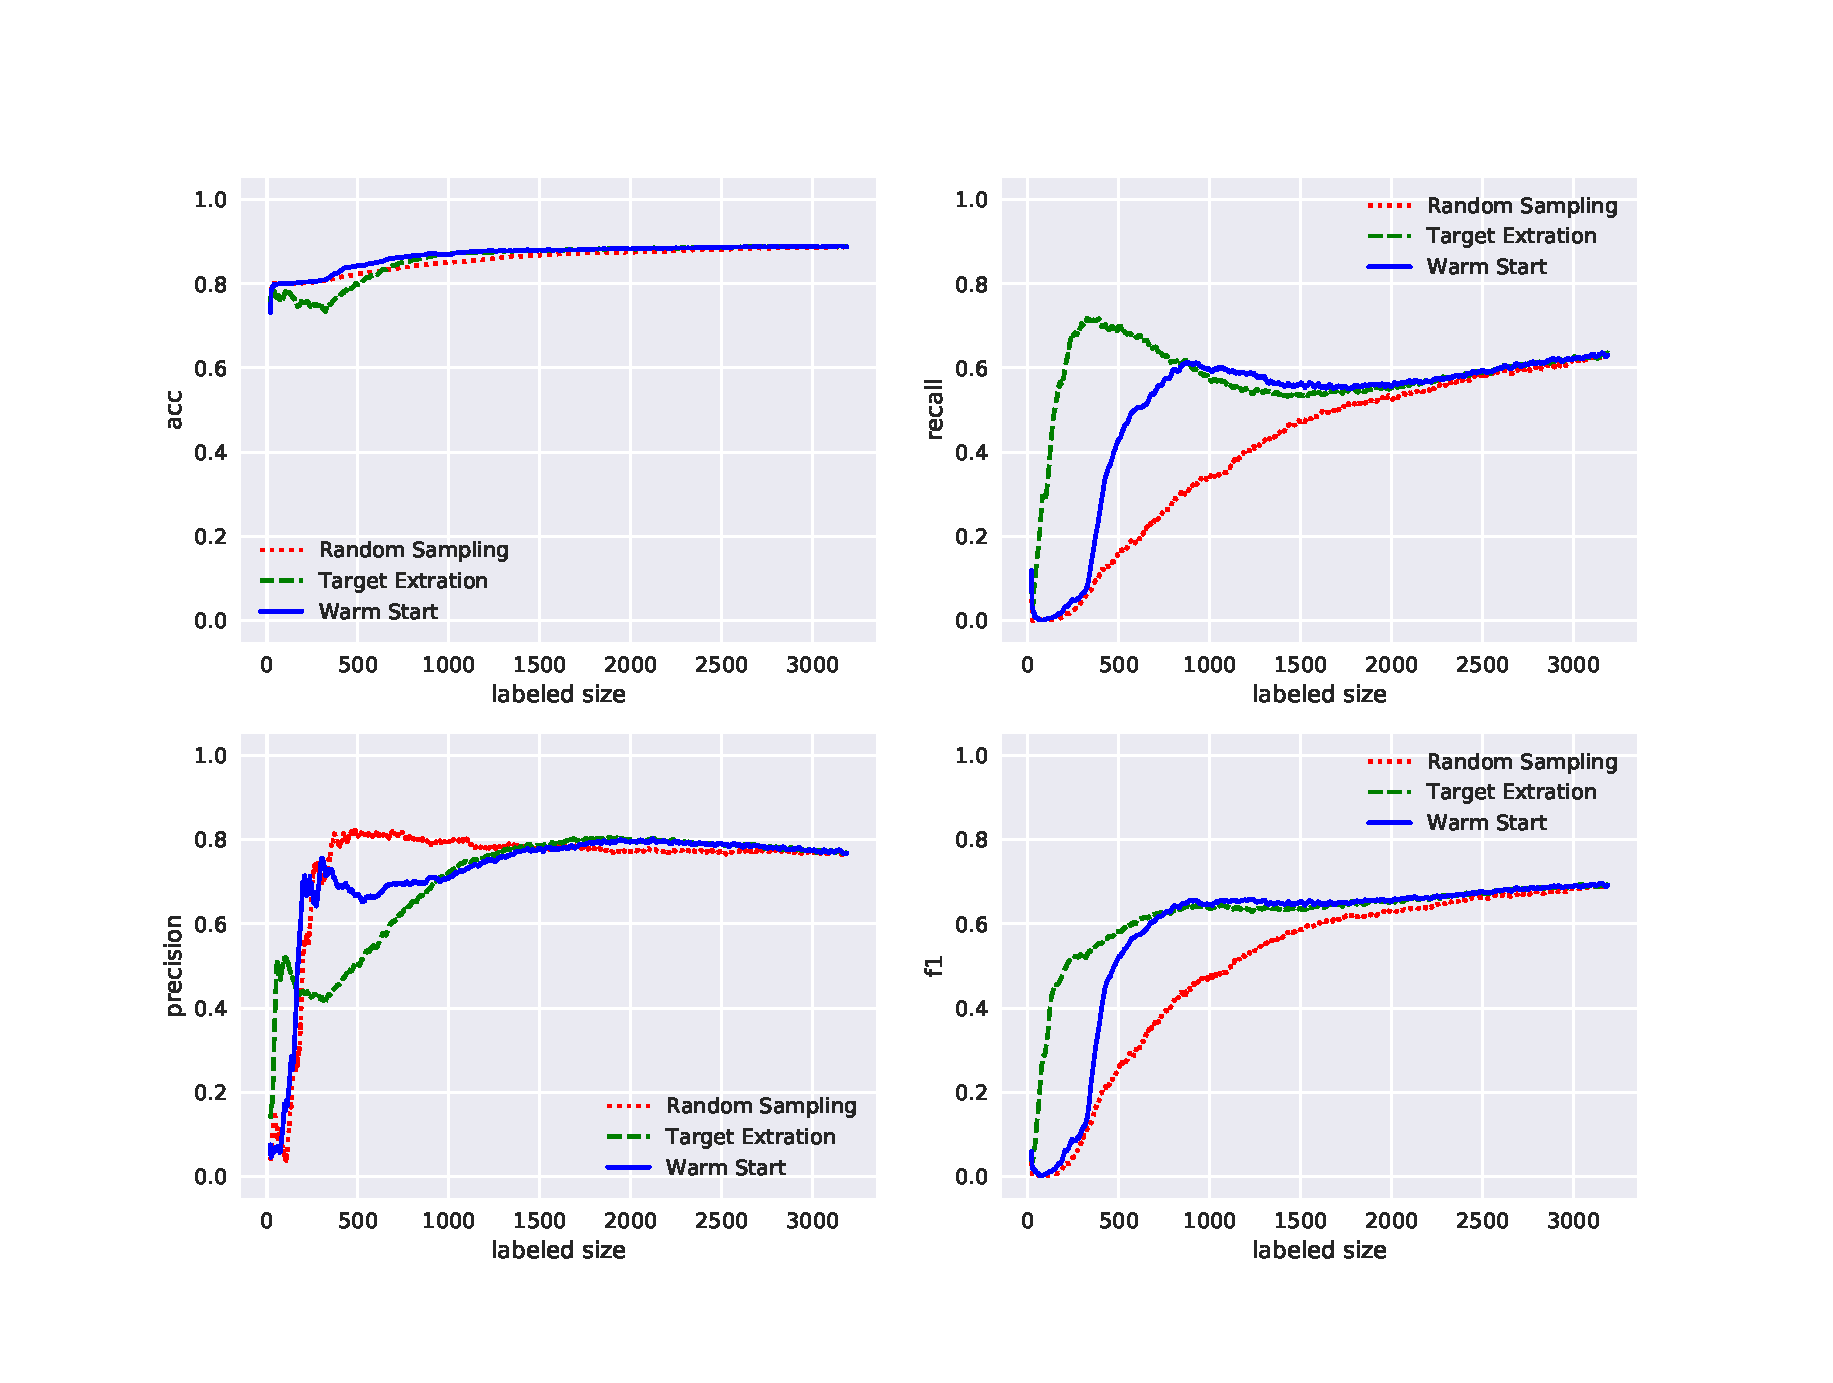
\includegraphics[width=0.9\textwidth]{resource/imdb/oracle_k-fold5}
\captionof{figure}{Metrics on Oracle Test Set}
\label{oracle2}
\end{figure*}

\begin{figure*}[!t]
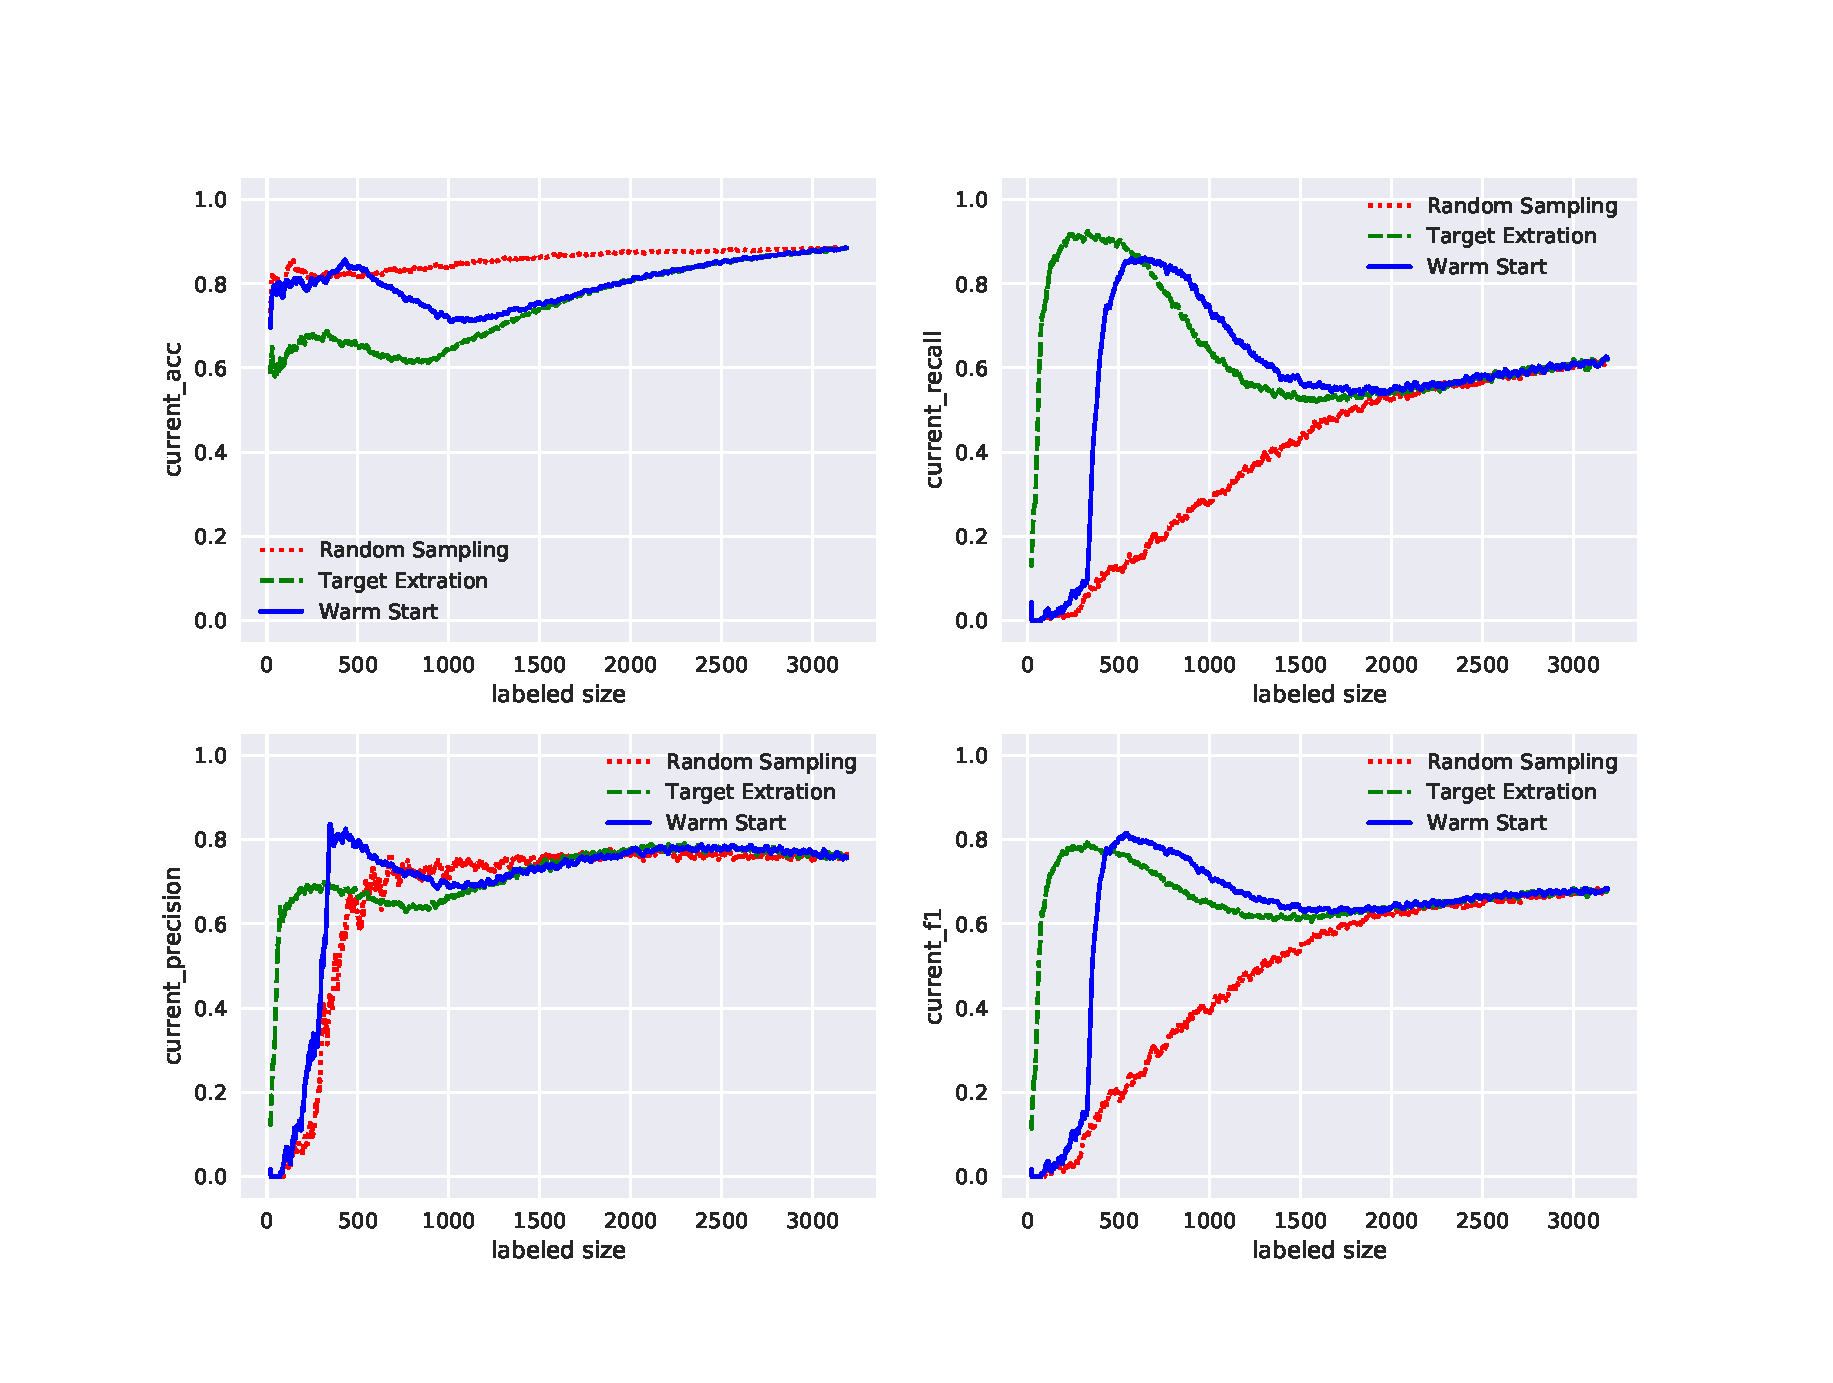
\includegraphics[width=0.9\textwidth]{resource/imdb/current_k-fold5}
\captionof{figure}{Metrics on Current Test Set}
\label{current2}
\end{figure*}

\begin{figure}[!t]
\includegraphics[width=0.4\textwidth]{resource/imdb/pos_coverage}
\captionof{figure}{Positive Coverage}
\label{pos_cov2}
\end{figure}

\begin{figure}[!t]
\includegraphics[width=0.4\textwidth]{resource/imdb/r_precision}
\captionof{figure}{R-Precision}
\label{rprecision2}
\end{figure}

\begin{figure}[!t]
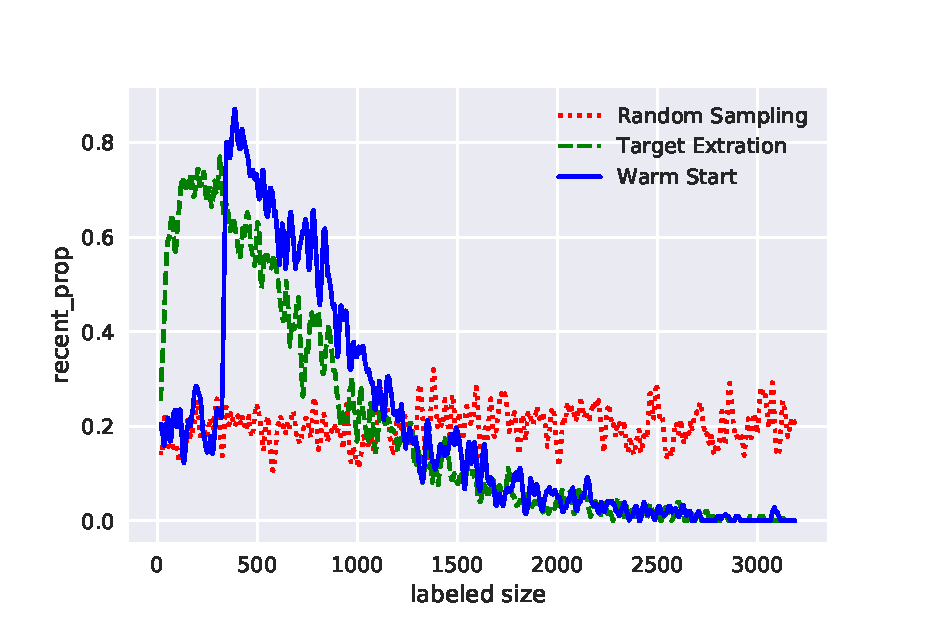
\includegraphics[width=0.4\textwidth]{resource/imdb/recent_prop}
\captionof{figure}{Recent Target Proporttion}
\label{recent2}
\end{figure}

\subsection{Results on Dataset 1}

In Figure~\ref{pos_cov1} showing positive coverage, we can see that
target-extraction works expectedly. On the other hand, in
Figure~\ref{oracle1}, since both accuracy and f1-score on oracle test
set show good results at the final step, we can assert that the model
is well trained. However, random sampling gives a much better learning
speed than target-extraction, since the labeled data does not have any
bias. On the other hand, in target-extraction, the model does not
learn well at the early phase, since the labeled data used to train is
biased towards target samples. As the model has found most of target
samples (aroud the step 600), non-target samples begin to increase in
the labeled data, and the model starts to learn the classification
task properly.  In the precision on the current test set (Figure
\ref{current1}), there is an obvious pit around the step 700. We call
it ``current precision pit''.  The reason of this pit is as follows.
At the early phase, the training data set is biased toward the target
data, and the model does not well trained.  However, the current test
set is also biased toward the target data, so the model shows good
performance on the current test set, and we cannot know that the model
is not well-trained only from the current test set metrics. At the
later phase, as the current test set gradually becomes balanced, these
metrics begin to go down, but when the model begins to learn the
classification task properly, the metrics go up again.

In Figure~\ref{rprecision1} showing R-precision, we can see that the
model shows poor R-precision compared with random sampling in early
steps, when the model is not well trained.  On the contrary, when the
model starts to perform well around step 700, R-precision of
target-extraction surpass that of random sampling, which indicates
that the model trained by target-extraction algorithm also provides a
better ranking. This satisfies our second purpose of providing a good
target likelihood ranking, so that we can switch from human annotation
to the prediction by the model.

The warm start method has shown a compromised result. Althought it do
not extract target data as fast as pure target-extraction method, it
was able to provide a much higher R-precision.

Figure~\ref{recent1}, which shows the recent labeled target
proportion, indicates the proportion of target samples in the recent
ten labeled data. Random sampling shows a relatively stable curve as
expected, while target-extraction picks much more target samples at
early steps, but the proportion goes down at later steps when less
target samples remain in unlabeled data. Since this is a metric which
can be known in real application, it provide a possibility to estimate
the target proportion of unlabeled data. Also, in warm start method,
%tajima: I didn't understand the next sentence.
it provided a priori of the whole unlabeled pool as expected.

\subsection{Results on Dataset 2}

Figure~\ref{oracle2} to \ref{recent2} show the result for the second
data set.  In Figure~\ref{current2}, although the current precision
pit came earlier and lasted for longer than in the previous experiment
with the balanced dataset, f1-scores on oracle test set and current
test set still converged, which means we can use current performance
to estimate oracle performance after the pit appears.

The f1-score on oracle test set of Dataset 1 (Figure~\ref{oracle2})
shows that the model with target-extraction method learned much slower
than with random sampling, due to the bias towards target
data. However, in unbalanced dataset, model with target-extraction
method learned much faster than random sampling. This is because the
model tried to fetch target data, which is minority in unlabeled data
pool, so that the model was able to learn on a more balanced dataset
than random sampling. In this way, target-extraction method not only
fetched target data faster, but contributed to model performance as
well for this data set where the target data is minority. Hence, we
can expect that if the target data is majority in the unlabeled pool,
the model will learn on a even more unbalanced dataset, and the
performance will go worse than random sampling.

Figure~\ref{rprecision2} shows that random sampling and
target-extraction on this unbalanced Dataset 2 gave the results
opposite to those on balanced Dataset 1.  It is easy to understand
because a well-learned model should provide a better ranking of target
likelihood.  We can also conclude that the warm start method gives a
compromised performance of R-precision on both balanced and unbalanced
datasets.

\section{Conclusion}

We defined a new problem called target-extraction-learning. The
purpose is to extract target data faster, and we propose a two-phase
approach. At the early phase, the system queries samples most likely
to be a target data for annotation, and at the later phase, we switch
from human annotation to the prediction by the model. We also analyze
the difficulty in the model performance estimation due to the bias
towards target data in the training data set. To handle this
difficulty, we use a phenomena we found in our experiiments. We can
observe a ``current precision pit'' in precision curve on current test
set, and we are able to estimate the model performance since the
results on current test set and oracle test set begin to converge
after striding over the pit. Finally, to handle the dilemma between
model performance and target extraction, we proposed a compromised
approach with a warm start of random sampling, and it gives
compromised results, both on balanced and unbalanced data.

However, the ``current precision pit'' can only be observed after the
model is well-trained.  If the model cannot be well trained on a
certain dataset, the pit will not appear.  We still need a way to
estimate the performance even in such cases.  In addition, estimation
using the experimental phenomena is still ambiguous, and it is better
to give more statistical evidence, such as the expectation and
variance to the performance of current model.

\section{Acknowledgment}

This work was supported by JST CREST (JPMJCR16E3),and JSPS KAKENHI Grant
Numbers 18H03245, 16K12430, and 18K11425.

%\vspace{30mm} <- Use if the body is too close to the references.
\vspace{2em}

% \bibliographystyle{plain}
% \bibliography{references}

\begin{thebibliography}{1}

\bibitem{enumerate}
Patrick J\"{o}rger, Yukino Baba, and Hisashi Kashima.
\newblock Learning to enumerate.
\newblock {\em Artificial Neural Networks and Machine Learning}, 2016.

\bibitem{predictive}
Y.~Baba et al.
%  H. Kashima, Y.~Nohara, E.~Kai, P.~Ghosh, R.~Islam, A.~Ahmed,
%  M.~Kuruda, S.~Inoue, T.~Hiramatsu, M.~Kimura, S.~Shimizu, K.~Kobayashi,
%  K.~Tsuda, M.~Sugiyama, M.~Blondel, N.~Ueda, M.~Kitsuregawa, and N.~Nakashima.
\newblock Predictive approaches for low-cost preventive medicine program in
  developing countries.
\newblock {\em Proc.\ of KDD}, pages 1681--1690, 2015.

\bibitem{survey}
Anita Krishnakumar.
\newblock Active learning literature survey.
\newblock 2007.

\bibitem{uncertainty}
David~D. Lewis and William~A. Gale.
\newblock A sequential algorithm for training text classifiers.
\newblock {\em Proc.\ of SIGIR},
  1994.

\bibitem{sklearn}
F.~Pedregosa et al.
% G.~Varoquaux, A.~Gramfort, V.~Michel, B.~Thirion, O.~Grisel,
% M.~Blondel, P.~Prettenhofer, R.~Weiss, V.~Dubourg, J.~Vanderplas, A.~Passos,
%  D.~Cournapeau, M.~Brucher, M.~Perrot, and E.~Duchesnay.
\newblock Scikit-learn: Machine learning in python.
\newblock {\em Journal of Machine Learning Research}, 12:2825--2830, 2011.

\end{thebibliography}

\end{document}
